\chapter{Análisis Experimental}\label{chapter:experiments}

En este capítulo se evalúa la capacidad de nuestro sistema de optimización para resolver problemas de clasificación y lograr buenos resultados según métricas de precisión y equidad.
La experimentación realizada consiste de dos etapas.
Inicialmente se analiza la capacidad de la primera fase del sistema para obtener un conjunto de modelos base lo suficientemente diverso como para que ensamblar sus predicciones resulte en un modelo de mayor precisión que los modelos base.
Finalmente, se estudia si el algoritmo propuesto permite encontrar formas de ensamblar los modelos base resultantes de la primera etapa de manera tal que se obtengan valores satisfactorios tanto de precisión como en las métricas de equidad.

\section{Marco Experimental}\label{section:experimental-framework}

Las dos etapas en las que queda divida nuestra experimentación se describen a continuación

La \textbf{primera etapa experimental} tiene como objetivo estudiar la capacidad del sistema de producir un conjunto de modelos base que, al ser ensamblado, pueda generalizar y obtener mejores resultados que dichos modelos base.
Adicionalmente, se desea estudiar que influencia tienen las distintas métricas de diversidad utilizadas en esta capacidad del sistema.

Para estimar el mejor rendimiento obtenible a partir de ensamblar el conjunto de modelos base encontrado, dos medidas son propuestas a continuación.
Estas medidas estiman el rendimiento que logran modelos de ensemble artificiales, estos son modelos de ensemble que conocen los resultados correctos a priori, y por tanto son modelos que no tienen utilidad real fuera de ser utilizados con propósitos de comparación.
Llamaremos a dichos ensembles: \emph{Oráculo Optimista} y \emph{Oráculo Sobreajustado}.

\begin{description}

\item[Oráculo Optimista.]
Este modelo oráculo devuelve la etiqueta correcta si al menos uno de los modelos base predijo dicha etiqueta.
La única forma de que este modelo falle es si ninguno de los modelos base fue capaz de sugerir la etiqueta correcta.

\begin{equation*}
O_{optimista}^{(i)}(M) =
    \begin{cases}
        y_i & \textrm{si $y_i \in \{\,y^{(j)}_i \mid m^{(j)} \in M \,\}$} \\
        y^{(0)}_i & \textrm{en otro caso} \\
    \end{cases}
\end{equation*}

Los resultados alcanzados por este ensemble reflejan el grado de cobertura de los modelos base sobre la colección de evaluación, esto es, cuantos ejemplos son correctamente predichos por al menos uno de los clasificadores base.

\item[Oráculo Sobre-ajustado.]
Este modelo oráculo computa todas las combinaciones de salidas de los modelos base y asigna a cada combinación la etiqueta mas frecuente encontrada en el conjunto correspondiente de etiquetas correctas.
Este modelo falla cuando la misma combinación de modelos base tiene que producir diferentes etiquetas para que todas las posibles entradas sean clasificadas correctamente.

\begin{equation*}
O_{sobreajustado}^{(i)}(M) =
    \textbf{max\_count}\left(\left\{\, y_k \,\middle\vert\, (x_k, y_k) \in D, \, \underset{m^{(j)} \in M}{\forall} y^{(j)}_k = y^{(j)}_i \,\right\}\right)
\end{equation*}

La función \textbf{max\_count} devuelve el elemento mas frecuente de la colección (en caso de un empate, siempre devuelve el primero que encuentra).

Los resultados que obtiene este ensemble, proveen una cota superior del mejor rendimiento que puede ser obtenido utilizando un conjunto de reglas \textbf{consistente} para ensamblar la colección de modelos base.

\end{description}

En esta primera etapa experimental se desea validar que nuestro sistema es capaz de generar modelos base en la primera fase que al ser ensamblados en la segunda fase dan lugar a un ensemble que obtiene mejores resultados sobre el conjunto de evaluación que cualquiera de los modelos base de los que se compone.
Para ello, los resultados obtenidos por el ensemble producido por nuestro sistema son comparados con los obtenidos por el mejor de los modelos base, y analizados respecto a los resultados obtenidos por el \emph{Oráculo Sobre-ajustado} descrito anteriormente.

Además, en esta etapa experimental se desea también comprobar la influencia de las diferentes métricas de diversidad utilizadas en la capacidad del sistema para producir modelos base que generalicen luego de ser ensamblados.
Con este propósito, se realiza un análisis de que tan bien los modelos base cubren el espacio de entrada de nuestro problema.
Para este análisis resulta de suma utilidad el concepto de \emph{Oráculo Optimista}, el cual nos darán información acerca de la influencia de las distintas métricas de diversidad en la distribución de los distintos modelos base sobre el espacio de entrada de nuestros datos.
Los resultados obtenidos por nuestro sistema son entonces comparados con aquellos del \emph{Oráculo Optimista} para cada una de las métricas de diversidad utilizadas.

Finalmente, se analiza también en esta etapa el comportamiento del sistema bajo diferentes combinaciones de otros hiperparámetros como la cantidad de modelos base.
La mejor configuración de dichos hiperparámetros, incluyendo la métrica de diversidad que mejores resultados proporciona al sistema, son utilizados en la segunda etapa experimental.

La \textbf{segunda etapa experimental} consiste en el estudio de la capacidad del sistema para lograr producir modelos de ensemble que son precisos de acuerdo a una función de perdida determinada y justos según una o varias métricas de equidad. 
Con este fin se realiza una comparación entre los resultados obtenidos por nuestro sistema y los obtenidos por varios otros sistemas que resultan relevantes en la literatura para la solución de este problema.

En el contexto de mitigación de sesgos, múltiples métodos \emph{ad-hoc} o dependientes del modelo han sido propuestos.
Estos métodos tratan de forzar equidad durante el entrenamiento y guían el proceso de optimización de los parámetros para que los modelos resultantes sean efectivos y justos respecto a una métrica de equidad predeterminada.
Uno de los objetivos de esta etapa experimental es precisamente comprobar si nuestro sistema es lo suficientemente poderoso como para tener mejor rendimiento que estos sistemas que influencian directamente el entrenamiento de los modelos con objetivos de mejorar los resultados de equidad obtenidos.

Alternativamente existen estrategias en la literatura, agnósticas al modelo, para lograr resultados justos.
Algunas realizan un preprocesamiento sobre la colección de datos para luego poder ajustar un modelos a los mismos.
Otras, como \emph{Fair Bayesian Optimization}, realizan un ajuste de los hiperparámetros del modelo deseado.
Estas propuestas, al igual que la nuestra, son muy versátiles, pues no imponen restricciones sobre el tipo de modelo a utilizar.
Por tanto, es de interés el estudio del rendimiento de nuestro sistema frente a estos enfoques para lograr modelos eficaces y justos.

Además, una de las ventajas de nuestro sistema es que permite optimizar simultáneamente varias métricas de equidad.
Por lo que se contrastan los resultados de nuestro método en este escenario con los de \emph{Fair Bayesian Optimization}, el cual por sus características también permite múltiples restricciones de equidad.

Finalmente se desea estudiar la capacidad de nuestro sistema de encontrar diferentes balances de equidad y precisión, no solo cumplir con una restricción de equidad.
Para ello nuestro sistema es comparado con otros métodos de optimización multiobjetivo relevantes en la literatura y que han mostrado buenos resultados en la solución de este problema.

\subsection{Escenarios de Evaluación}\label{section:evaluation-scenaries}

La primera etapa experimental evalúa el sistema en la tarea \emph{HAHA 2019}(\textit{Humor Analysis based on Human Annotation}), con marco en el evento \textit{IberLEF 2019} \parencite{chiruzzo2019overview}.
El proceso de evaluación consiste primero de la ejecución de la primera fase de nuestro sistema, esto es, la exploración del espacio de modelos y obtención del conjunto de modelos base a ser ensamblados.
Posteriormente la segunda fase de nuestro sistema es ejecutada, utilizando como única función objetivo la función de perdida que fue utilizada en la obtención de los modelos base.
La función objetivo a optimizar en ambas fases del sistema es la precisión del sistema.
Como parte de esta etapa se realizan múltiples ejecuciones con diferentes configuraciones de hiperparámetros.
La configuración de hiperparámetros para la cual se observen los mejores resultados en esta etapa, sera la utilizada en la segunda etapa experimental, como se describe a continuación.

La segunda etapa experimental consiste en la ejecución de extremo a extremo de nuestro sistema, utilizando la colección de datos \emph{Adult}~\parencite{ucidata} como escenario de evaluación.
En esta etapa se utiliza la mejor configuración de hiperparámetros acorde a los resultados de la primera fase, es relevante destacar que entre estos hiperparámetros preseleccionados en la etapa anterior se encuentran la medida de diversificación a utilizar en la selección de modelos base y la cantidad máxima de estos.
Ambas fases optimizan la precisión del modelo, en particular la segunda fase incorpora al proceso de optimización métricas de equidad, dígase \emph{Statistical Parity} y \emph{Equalized Opportunity}, como funciones objetivo adicionales a optimizar simultáneamente con la precisión.

\subsection{Corpus de Evaluación}\label{section:evaluation-corpus}

Dos conjuntos de datos son utilizados para la evaluación del sistema en los experimentos realizados.

\begin{description}

\item[HAHA 2019.]
Colección de datos utilizada en la tarea \emph{HAHA 2019} (\emph{Humor Analysis based on Human Annotation}), con marco en \emph{IberLEF 2019} \parencite{chiruzzo2019overview}.
El corpus contiene $30\,000$ tweets en Español clasificados manualmente, de los cuales $24\,000$ son para entrenamiento y $6\,000$ para evaluación.
Cada uno de estos tweets es clasificado en \emph{gracioso} o \emph{no-gracioso}.

La colección de datos es anotada a partir de asignar una clasificación de \emph{gracioso} o \emph{no-gracioso} a cada tweet, en caso de ser \emph{gracioso} se da una puntuación de $[1,5]$ de cuan \emph{gracioso} es dicho tweet.

\begin{table}[h]
    \centering
    \begin{tabular}{lccc}
    \toprule
                            & Entrenamiento & Evaluación & Total   \\\midrule
        Tweets              & 24\,000       & 6\,000     & 30\,000 \\
        Graciosos           & 9\,253        & 2\,342     & 11\,595 \\
        No graciosos        & 14\,757       & 3\,658     & 18\,405 \\
        Puntuación promedio & 2.04          & 2.03       & 2.04    \\\midrule
        Total de Votos      & 59\,440       & 13\,605    & 73\,045 \\
        Votos 1             & 19\,063       & 4\,818     & 23\,881 \\
        Votos 2             & 14\,713       & 3\,777     & 18\,490 \\
        Votos 3             & 10\,206       & 2\,649     & 12\,855 \\
        Votos 4             &  4\,493       & 1\,122     &  5\,615 \\
        Votos 5             &  1\,305       &    275     &  1\,580 \\
    \bottomrule
    \end{tabular}
    \caption{Composición de los datos según la cantidad de votos para cada clase.}
    \label{table:haha2019info}
\end{table}

\item[Adult.]
La colección de datos \emph{Adult} \parencite{ucidata} presenta información extraída del censo de 1994 en los Estados Unidos por Barry Becker.
Los datos contienen detalles personales de los individues, tales como nivel de educación, horas de trabajo a la semana, raza, sexo, etc.
El objetivo es predecir si el individuo ganará un salario mayor a \texttt{\$50K} al año.
Hay un total de $48\,842$ filas de datos, y de estas, $3\,620$ contienen casillas con valores desconocidos, dejando $45\,222$ filas completas.
Existen dos clases en las cuales clasificar a los individuos dependiendo de su salario anual, estas son, \texttt{>50K} o \texttt{$\leq$50K}.
Las clases están desbalanceadas, con una tendencia hacia la etiqueta \texttt{<50K}, la cual representa aproximadamente el $75\%$ de los ejemplos.

\end{description}

\subsection{Configuración Experimental}\label{section:experimental-setup}

En todos los experimentos, el sistema fue configurado para permitir que cada fase ejecutara a lo sumo $10\,000$ iteraciones o por una hora.
Los parámetros de búsqueda de AutoGOAL fueron los siguientes:
\begin{itemize}
    \item \texttt{popsize=50}
    \item \texttt{selection=10}
    \item \texttt{cross\_validation\_steps=3}
    \item \texttt{validation\_split=0.3}
\end{itemize}

Debido a limitaciones de infraestructura, los algoritmos de aprendizaje profundo fueron excluidos del conjunto de algoritmos disponibles para AutoGOAL.
Por ejemplo, flujos basados en \emph{Keras} y \emph{BERT} fueron excluidos y fundamentalmente flujos basados en \emph{ScikitLearn} fueron utilizados.

No incluir los algoritmos de aprendizaje profundo en la configuración experimental puede tener un impacto negativo en el rendimiento máximo que puede ser alcanzado por el sistema.
Es decir, la precisión del sistema no puede ser comparada directamente con otras soluciones reportadas, en términos de magnitud, pues aquellas soluciones que utilizan técnicas de aprendizaje profundo tienen una ventaja inherente en problemas donde modelos más simples no son tan competitivos.
Sin embargo, la ausencia de estos algoritmos no deberían afectar la capacidad del sistema de mejorar el rendimiento respecto a los modelos base encontrados en la primera fase.
Por tanto, si el sistema es capaz de mejorar el rendimiento de los modelos base, entonces el rendimiento del sistema se espera que mejore aún más una vez que las arquitecturas de aprendizaje profundo sean compatibles.
Esto se espera que ocurra no solo porque los modelos base ahora tendrían mejor rendimiento, sino también porque arquitecturas de ensemble mas poderosas serían añadidas al mismo tiempo sin esfuerzo alguno.
AutoGOAL ya ha probado lograr resultados competitivos cuando es configurado correctamente \parencite{estevez2020automatic}.
Además, es importante destacar que, en el caso en que se optimiza buscando un buen balance entre la precisión y las métricas de equidad, por ejemplo en la segunda fase de nuestro sistema, no necesariamente modelos mas poderosos (como los de aprendizaje profundo) implican mejores resultados en dicho balance.
Por tanto, la comparativa con otros métodos de mitigación no debería verse afectada significativamente.

\subsubsection{Biblioteca}\label{section:library}

El sistema propuesto en este trabajo es parte de la biblioteca en desarrollo \texttt{BFair}\footnote{https://github.com/bfair-ml/bfair}
La biblioteca tiene como objetivo atacar los problemas de sesgos que emergen de entrenar modelos de \emph{Aprendizaje Automático} que en datos que muestran sesgos de los humanos.

\todo[inline]{Aquí quizas puedes poner un ejemplo de cómo queda un llamado a la interfaz para resolver Adult. En plan, la parte de cargar los datos la pones como una funcion maquica y abajo lo que pones es el código de python con los hiperparámetros que tocan.}

\subsubsection{Hardware}\label{section:hardware}

Los experimentos fueron ejecutados en un equipo con las siguientes propiedades:
CPU Intel Core i9-9900K (-MT-MCP-) con velocidad máxima de 3651/5000 MHz, cache de 16384KB y RAM de 64GB.

\section{Primera Etapa Experimental}\label{section:experiments-first-phase}

A continuación, la sección~\ref{section:results-first-phase} muestra los resultados de los obtenidos a partir de realizar los experimentos de la forma descrita en la sección~\ref{section:experimental-framework} para la tarea \emph{HAHA 2019}.
Luego la sección~\ref{section:discussion-first-phase} realiza un análisis en profundidad de dichos resultados y arriba a conclusiones a partir de los mismos.

\subsection{Resultados}\label{section:results-first-phase}

Las tablas~\ref{table:haha-5},~\ref{table:haha-20},~\ref{table:haha-50},~\ref{table:haha-100} resumen los resultados obtenidos por el sistema en la tarea \emph{HAHA 2019}, para configuraciones con número máximo de clasificadores base siendo $5$, $20$, $50$ y $100$ respectivamente.
El sistema fue configurado para utilizar en ambas fases una función de pérdida basada en $F_1$, la cual fue propuesta como métrica de puntuación en la descripción de la tarea.
Cinco estrategias de control de población fueron evaluadas con el objetivo de establecer comparaciones, de las cuales dos son las métricas de diversidad discutidas en la sección~\ref{section:diversity-meassures}, y las tres restantes son las implementaciones de referencia del método~\ref{code:reselect} presentados en la sección~\ref{section:first-phase}.
Cada tabla muestra la métrica $F_1$ alcanzada por:
(i) los oráculos optimista y sobreajustados (sección~\ref{section:experimental-framework});
(ii) el modelo obtenido a partir de ensamblar los modelos base~(sección~\ref{section:second-phase}); y,
(iii) el mejor modelo base encontrado~(sección~\ref{section:first-phase}).
Además, el tipo de algoritmo de ensemble utilizado por el mejor de los modelos de ensemble encontrados es adicionado al final de cada tabla.


%For the experiments reported next, only the training collection is used to tune the system.
%The testing collection is used to report unbiased scores.
%
%The training collection was divided into three cross-validation folds for the first phase, using a 30\% validation split.
%Additionally, it was also divided into two pre-established training and valid collections using a 30\% validation split.
%These pre-established collections were the ones used to measure diversity in the first phase
%and the ensembling performance in the second phase.
%\textcolor{black}{
%The original testing collection of the corpus was used to report the final testing results.
%This collection was not used during training.
%}

\begin{table}[H]
    \centering
    \resizebox{\textwidth}{!}{
    \begin{tabular}{lccccc}
    \toprule
        & shuffle & arbitrary & best & disagreement & double-fault  \\ \midrule \midrule
        oráculo optimista ($F_1$)  & 0.996   & 0.917   & 0.893   & 1.000   & 0.970 \\
        oráculo sobreajustado ($F_1$)  & 0.715   & 0.711   & 0.744   & 0.748   & 0.754 \\ \midrule
        % oráculo optimista ($acc.$)  & 0.997   & 0.937   & 0.915   & 1.000   & 0.977 \\
        % oráculo sobreajustado ($acc.$)  & 0.794   & 0.794   & 0.816   & 0.795   & 0.818 \\ \midrule
        $A^*$ ($F_1$, entrenamiento)  & 0.989   & 0.973   & 0.945   & 0.846   & 0.876 \\
        $A^*$ ($F_1$, evaluación)  & 0.690   & 0.711   & 0.722   & 0.749   & 0.757 \\
        $E^*$ ($F_1$, entrenamiento)  & 0.913   & 0.961   & 0.917   & 0.846   & 0.941 \\
        $E^*$ ($F_1$, evaluación)  & 0.731   & 0.726   & 0.755   & 0.749   & 0.761 \\
        \midrule
        % delta (evaluación)  & 0.040   & 0.015   & 0.033   & 0.000   & 0.004 \\
        % delta (entrenamiento)  & -0.076   & -0.012   & -0.027   & 0.000   & 0.065 \\ \midrule
        tipo de ensemble & voting & learning & learning & voting & voting \\
    \bottomrule
    \end{tabular}}
    \caption{HAHA 2019. Máximo número de modelos base es 5.
    Cada columna muestra el resultado obtenido utilizando la estrategia de selección de modelos base correspondiente.
    $A^*$ y $E^*$ representan el modelo base de mejor rendimiento y la mejor configuración de ensemble encontrada, respectivamente.
    Tipos de ensemble: \emph{voting}, \emph{overfit}, y \emph{learning}, representan a \emph{Voting Classifier}, \emph{Overfitted Voting Classifier}, y \emph{ML Voting Classifier}, respectivamente.}
    \label{table:haha-5}
\end{table}

\begin{table}[H]
    \centering
    \resizebox{\textwidth}{!}{
    \begin{tabular}{lccccc}
    \toprule
        & shuffle & arbitrary & best & disagreement & double fault  \\ \midrule \midrule
        oráculo optimista ($F_1$) & 1.000  & 1.000  & 0.936  & 1.000  & 0.998 \\
        oráculo sobreajustado ($F_1$) & 0.729  & 0.771  & 0.831  & 0.735  & 0.889 \\ \midrule
        % oráculo optimista ($acc.$) & 1.000  & 1.000  & 0.951  & 1.000  & 0.998 \\
        % oráculo sobreajustado ($acc.$) & 0.803  & 0.832  & 0.870  & 0.789  & 0.917 \\ \midrule
        $A^*$ ($F_1$, entrenamiento) & 0.876  & 0.901  & 0.855  & 0.875  & 0.856 \\
        $A^*$ ($F_1$, evaluación) & 0.705  & 0.721  & 0.759  & 0.732  & 0.755 \\
        $E^*$ ($F_1$, entrenamiento) & 0.870  & 0.930  & 0.883  & 0.875  & 0.942 \\
        $E^*$ ($F_1$, evaluación) & 0.719  & 0.740  & 0.765  & 0.732  & 0.767 \\ \midrule
        % delta (evaluación) & 0.014  & 0.018  & 0.005  & 0.000  & 0.012 \\
        % delta (entrenamiento) & -0.006  & 0.030  & 0.029  & 0.000  & 0.086 \\ \midrule
        tipo de ensemble & learning & overfit & voting & learning & voting \\
    \bottomrule
    \end{tabular}}
    \caption{HAHA 2019. Máximo número de modelos base es 20.
    Cada columna muestra el resultado obtenido utilizando la estrategia de selección de modelos base correspondiente.
    $A^*$ y $E^*$ representan el modelo base de mejor rendimiento y la mejor configuración de ensemble encontrada, respectivamente.
    Tipos de ensemble: \emph{voting}, \emph{overfit}, y \emph{learning}, representan a \emph{Voting Classifier}, \emph{Overfitted Voting Classifier}, y \emph{ML Voting Classifier}, respectivamente.}
    \label{table:haha-20}
\end{table}

\begin{table}[H]
    \centering
    \resizebox{\textwidth}{!}{
    \begin{tabular}{lccccc}
    \toprule
        & shuffle & arbitrary & best & disagreement & double fault  \\ \midrule \midrule
        oráculo optimista ($F_1$) & 1.000  & 1.000  & 0.978  & 1.000  & 1.000 \\
        oráculo sobreajustado ($F_1$) & 0.953  & 0.950  & 0.927  & 0.996  & 0.969 \\ \midrule
        % oráculo optimista ($acc.$) & 1.000  & 1.000  & 0.983  & 1.000  & 1.000 \\
        % oráculo sobreajustado ($acc.$) & 0.965  & 0.961  & 0.944  & 0.997  & 0.977 \\ \midrule
        $A^*$ ($F_1$, entrenamiento) & 1.000  & 0.928  & 0.877  & 0.857  & 0.913 \\
        $A^*$ ($F_1$, evaluación) & 0.639  & 0.720  & 0.720  & 0.750  & 0.749 \\
        $E^*$ ($F_1$, entrenamiento) & 1.000  & 0.924  & 0.921  & 1.000  & 0.923 \\
        $E^*$ ($F_1$, evaluación) & 0.741  & 0.736  & 0.731  & 0.747  & 0.756 \\
        \midrule
        % delta (evaluación) & 0.102  & 0.015  & 0.012  & -0.003  & 0.006 \\
        % delta (entrenamiento) & 0.000  & -0.004  & 0.044  & 0.143  & 0.010 \\ \midrule
        tipo de ensemble & overfit & learning & voting & overfit & voting \\
    \bottomrule
    \end{tabular}}
    \caption{HAHA 2019. Máximo número de modelos base es 50.
    Cada columna muestra el resultado obtenido utilizando la estrategia de selección de modelos base correspondiente.
    $A^*$ y $E^*$ representan el modelo base de mejor rendimiento y la mejor configuración de ensemble encontrada, respectivamente.
    Tipos de ensemble: \emph{voting}, \emph{overfit}, y \emph{learning}, representan a \emph{Voting Classifier}, \emph{Overfitted Voting Classifier}, y \emph{ML Voting Classifier}, respectivamente.}
    \label{table:haha-50}
\end{table}

\begin{table}[H]
    \centering
    \resizebox{\textwidth}{!}{
    \begin{tabular}{lccccc}
    \toprule
        & shuffle & arbitrary & best & disagreement & double fault  \\ \midrule \midrule
        oráculo optimista ($F_1$) & 1.000  & 1.000  & 0.997  & 1.000  & 1.000 \\
        oráculo sobreajustado ($F_1$) & 0.988  & 0.992  & 0.984  & 0.998  & 0.988 \\ \midrule
        % oráculo optimista ($acc.$) & 1.000  & 1.000  & 0.997  & 1.000  & 1.000 \\
        % oráculo sobreajustado ($acc.$) & 0.991  & 0.994  & 0.988  & 0.998  & 0.991 \\ \midrule
        $A^*$ ($F_1$, entrenamiento) & 0.998  & 0.856  & 0.853  & 0.902  & 0.920 \\
        $A^*$ ($F_1$, evaluación) & 0.683  & 0.748  & 0.759  & 0.745  & 0.750 \\ 
        $E^*$ ($F_1$, entrenamiento) & 1.000  & 1.000  & 1.000  & 0.970  & 0.940 \\
        $E^*$ ($F_1$, evaluación) & 0.756  & 0.745  & 0.761  & 0.728  & 0.743 \\
        \midrule
        % delta (evaluación) & 0.073  & -0.003  & 0.002  & -0.017  & -0.007 \\
        % delta (entrenamiento) & 0.002  & 0.144  & 0.147  & 0.069  & 0.020 \\ \midrule
        tipo de ensemble & overfit & overfit & overfit & learning & voting \\
    \bottomrule
    \end{tabular}}
    \caption{HAHA 2019. Máximo número de modelos base es 100.
    Cada columna muestra el resultado obtenido utilizando la estrategia de selección de modelos base correspondiente.
    $A^*$ y $E^*$ representan el modelo base de mejor rendimiento y la mejor configuración de ensemble encontrada, respectivamente.
    Tipos de ensemble: \emph{voting}, \emph{overfit}, y \emph{learning}, representan a \emph{Voting Classifier}, \emph{Overfitted Voting Classifier}, y \emph{ML Voting Classifier}, respectivamente.}
    \label{table:haha-100}
\end{table}


Como puede observarse, \textbf{
los mejores resultados fueron obtenidos cuando el máximo número de clasificadores base esta entre 20 y 50 y la estrategia de selección de modelos base es \emph{double-fault}.
}
A continuación, la sección~\ref{section:discussion-first-phase} profundiza en los resultados presentados en esta sección~\ref{section:results-first-phase}.

\subsection{Discusión}\label{section:discussion-first-phase}

Algunos patrones interesantes pueden ser observados a partir de analizar el rendimiento de los ensembles oráculo para diferentes estrategias de reselección de clasificadores base.
La tabla~\ref{table:oracle} resume el rendimiento de los oráculos optimista y sobreajustado en el conjunto de evaluación.
Algunos de estos patrones son presentados a continuación:

\begin{itemize}
    \item 
    La métrica \emph{disagreement} asegura la máxima cobertura del conjunto de entrenamiento sin importar el número de clasificadores base seleccionado.
    Esto tiene sentido dado que la medida de \emph{disagreement} premia la reselección de modelos que tienen predicciones con conflictos entre si.
    Observando el rendimiento del oráculo sobreajustado, se puede notar que a pesar de que provee un cubrimiento máximo, no hay un conjunto de reglas \textbf{consistente} que pueda ser aplicado para explotar dicho cubrimiento.
    
    \item
    La métrica \emph{double-fault} provee el rendimiento mas consistente para ambos el oráculo optimista y sobreajustado, en especial cuando el numero de clasificadores es bajo.
    Esto sugiere que la estrategia de diversificación basada en \emph{double-fault} puede proveer el mejor rendimiento en el subsecuente fase de ensamblado, dado que obtiene una mayor puntuación cuando se utiliza un conjunto de reglas consistente. 
    
    \item
    El cubrimiento mostrado por los ensembles oráculo se incrementa significativamente según se incrementa el número de clasificadores base, independientemente de la estrategia de reselección.
    Esto tiene sentido dado que un mayor conjunto de votantes incrementa la probabilidad de encontrar uno que correctamente clasifique los ejemplos de mayor conflicto si hay cierta diversidad entre los votantes.
    Esta idea es apoyada por el hecho de que la estrategia que reselecciona de forma golosa solo los modelos de mejor rendimiento es la que logra el menor cubrimiento (de acuerdo al ensemble optimista).
\end{itemize}

\begin{table}[H]
    \centering

    \begin{tabular}{lccccc}
    \toprule
        \multicolumn{6}{c}{Oráculo Optimista ($F_1$)} \\ \midrule
        n-clasificadores & shuffle & arbitrary & best & disagreement & double fault  \\ \midrule \midrule
        5   & 0.996 & 0.917 & 0.893 & 1.000 & 0.970 \\
        20  & 1.000 & 1.000 & 0.936 & 1.000 & 0.998 \\
        50  & 1.000 & 1.000 & 0.978 & 1.000 & 1.000 \\
        100 & 1.000 & 1.000 & 0.997 & 1.000 & 1.000 \\
    \bottomrule
    \end{tabular}

    \begin{tabular}{lccccc}
    \toprule
        \multicolumn{6}{c}{Oráculo Sobreajustado ($F_1$)} \\ \midrule
        n-clasificadores & shuffle & arbitrary & best & disagreement & double fault  \\ \midrule \midrule
        5   & 0.715 & 0.711 & 0.744 & 0.748 & 0.754 \\
        20  & 0.729 & 0.771 & 0.831 & 0.735 & 0.889 \\
        50  & 0.953 & 0.950 & 0.927 & 0.996 & 0.969 \\
        100 & 0.988 & 0.992 & 0.984 & 0.998 & 0.988 \\
    \bottomrule
    \end{tabular}

    \caption{Resumen de las métricas en los oráculos para cada estrategia de selección de modelos base según el numero máximo de clasificadores base se incrementa.}
    \label{table:oracle}
\end{table}

La tabla~\ref{table:delta} resume las diferencias entre el rendimiento logrado por el mejor ensemble encontrado $E^*$ y el mejor modelo base $A^*$, en ambas la colección de entrenamiento y de evaluación.
Es notable que los modelos de ensemble son capaces de sobrepasar a sus modelos base en la colección de entrenamiento, incluso cuando algunas estrategias requieren un mayor numero de modelos base para lograr esto.
La estrategia de \emph{double-fault} es capaz de mejorar el rendimiento incluso con un numero bajo de clasificadores base.
Esto tiene sentido dado que esta estrategia penaliza al sistema por construir una colección en la cual todos los modelos base fallen en los mismos ejemplos.
Por tanto, estos resulta en una colección de modelos base, en la cual cada modelo arregla los fallos del otro.
Este comportamiento es diferente al que muestra la estrategia de \emph{disagreement}, esta premia a los modelos base por tener diferentes predicciones independientemente de si estas eran correctas o incorrectas.
Esto puede llevar a situaciones en las cuales es difícil para el ensemble decidir en cual de los modelos base confiar, especialmente si el numero de modelos base es muy bajo.

Aun mas importante, la tabla~\ref{table:delta} también muestra que la optimización de ensemble es capaz de producir ensembles que generalizan mejor que sus modelos base, es decir, los ensembles tienen mejor rendimiento en el conjunto de evaluación.
Esto es particularmente cierto cuando el numero de clasificadores base no es muy grande. Según incrementa el numero de clasificadores base, también lo hace el numero de diferentes combinaciones, y por tanto, el ensemble es mas susceptible a sobre-ajustar el conjunto de entrenamiento.

\begin{table}[H]
    \centering

    \begin{tabular}{lccccc}
    \toprule
        \multicolumn{6}{c}{$(E^* - A^*)$ en entrenamiento} \\ \midrule
        n-clasificadores & shuffle & arbitrary & best & disagreement & double fault  \\ \midrule \midrule
        5  & \cellcolor{red!25}{-0.076}   & \cellcolor{red!25}-0.012   & \cellcolor{red!25}-0.027   & \cellcolor{yellow!25}0.000   & \cellcolor{green!25}0.065 \\
        20 & \cellcolor{red!25}-0.006  & \cellcolor{green!25}0.030  & \cellcolor{green!25}0.029  & \cellcolor{yellow!25}0.000  & \cellcolor{green!25}0.086 \\
        50 & \cellcolor{yellow!25}0.000  & \cellcolor{red!25}-0.004  & \cellcolor{green!25}0.044  & \cellcolor{green!25}0.143  & \cellcolor{green!25}0.010 \\
        100 & \cellcolor{green!25}0.002  & \cellcolor{green!25}0.144  & \cellcolor{green!25}0.147  & \cellcolor{green!25}0.069  & \cellcolor{green!25}0.020 \\
    \bottomrule
    \end{tabular}

    \begin{tabular}{lccccc}
    \toprule
        \multicolumn{6}{c}{$(E^* - A^*)$ en evaluación} \\ \midrule
        n-clasificadores & shuffle & arbitrary & best & disagreement & double fault  \\ \midrule \midrule
        5  & \cellcolor{green!25}0.040   & \cellcolor{green!25}0.015   & \cellcolor{green!25}0.033   & \cellcolor{yellow!25}0.000   & \cellcolor{green!25}0.004 \\
        20 & \cellcolor{green!25}0.014  & \cellcolor{green!25}0.018  & \cellcolor{green!25}0.005  & \cellcolor{yellow!25}0.000  & \cellcolor{green!25}0.012 \\
        50 & \cellcolor{green!25}0.102  & \cellcolor{green!25}0.015  & \cellcolor{green!25}0.012  & \cellcolor{red!25}-0.003  & \cellcolor{green!25}0.006 \\
        100 & \cellcolor{green!25}0.073  & \cellcolor{red!25}-0.003  & \cellcolor{green!25}0.002  & \cellcolor{red!25}-0.017  & \cellcolor{red!25}-0.007 \\
    \bottomrule
    \end{tabular}

    \caption{Resumen de la diferencia en rendimiento entre el mejor modelo base encontrado ($A^*$) y el ensemble correspondiente ($E^*$), para cada estrategia de selección de modelo base según incrementa el numero de clasificadores base.}
    \label{table:delta}
\end{table}

Algunas otras ideas que resaltan de la tabla~\ref{table:delta} se resumen a continuación:

\begin{itemize}
    \item
    Las métricas de diversidad, dígase \emph{disagreement} y \emph{double-fault}, tienen un mayor impacto en el rendimiento del ensemble en el conjunto de entrenamiento cuando el numero de clasificadores base es bajo.
    Esto tiene sentido dado que mientras menor cantidad de modelos en la colección de modelos base, mas difícil será encontrar una \textit{buena} selección de forma arbitraria.
    Sin embargo, las medidas de diversidad no parecen tener un impacto en las capacidades de generalización del ensemble.
    
    \item
    A la estrategia de \emph{disagreement} le resulta difícil mejorar el rendimiento, tanto en el conjunto de entrenamiento como en el de evaluación.
    Esto es particularmente cierto cuando el numero de clasificadores base es bajo.
    Esta estrategia no penaliza a los modelos por realizar predicciones erróneas y en su lugar los premia si sus predicciones son diferentes a la del resto de los clasificadores.
    Luego, es usual que el ensemble simplemente decida confiar en la predicción de solo uno de los clasificadores base, y por tanto el ensemble produce los mismos resultados que su mejor modelo base.
    Esto muestra que lograr el mejor cubrimiento de acuerdo al oráculo optimista, como lo logra la medida de \emph{disagreement}, no es necesariamente útil.
\end{itemize}

La tabla~\ref{table:performance} resume el rendimiento obtenido por el ensemble $E^*$ según el numero de clasificadores base y las estrategias de reselección cambian.
La estrategia de \emph{double-fault} siempre logra los mejores resultados, excepto en el ultimo escenario, en el cual el numero de clasificadores es el más alto.
En ese caso, aunque el ensemble obtuvo un mejor rendimiento que sus modelos base en la colección de entrenamiento, el numero alto de votantes puede haber afectado sus capacidades de generalización. dado que el espacio de posibles combinaciones de votantes es mayor.

\begin{table}[H]
    \centering
    
    \begin{tabular}{lccccc}
    \toprule
        \multicolumn{6}{c}{$E^*$ en entrenamiento} \\ \midrule
        n-clasificadores & shuffle & arbitrary & best & disagreement & double fault  \\ \midrule \midrule
        5 & 0.913 & {\bf 0.961} & 0.917 & 0.846 & 0.941 \\
        20 & 0.870 & 0.930 & 0.883 & 0.875 & {\bf 0.942} \\
        50 & {\bf 1.000} & 0.924 & 0.921 & {\bf 1.000} & 0.923 \\
        100 & {\bf 1.000} & {\bf 1.000} & {\bf 1.000} & 0.970 & 0.940 \\
    \bottomrule
    \end{tabular}

    \begin{tabular}{lccccc}
    \toprule
        \multicolumn{6}{c}{$E^*$ @ evaluación} \\ \midrule
        n-clasificadores & shuffle & arbitrary & best & disagreement & double fault  \\ \midrule \midrule
        5 & 0.731 & 0.726 & 0.755 & 0.749 & {\bf 0.761} \\
        20 & 0.719 & 0.740 & 0.765 & 0.732 & {\bf 0.767} \\
        50 & 0.741 & 0.736 & 0.731 & 0.747 & {\bf 0.756} \\
        100 & 0.756 & 0.745 & {\bf 0.761} & 0.728 & 0.743 \\
    \bottomrule
    \end{tabular}

    \caption{Resumen del rendimiento obtenido por el ensemble ($E^*$) en el conjunto de entrenamiento y evaluación, para cada estrategia de selección de modelos base según el numero maximo de clasificadores incrementa.}
    \label{table:performance}
\end{table}

Como es de esperarse, la ausencia de algoritmos de aprendizaje profundo en el conjunto de métodos disponibles tuvo un impacto negativo en el mayor rendimiento alcanzado.
% Our best performing architecture achieves $0.767$ $F_1$ while the best solution reported in the official HAHA 2019 challenge is $0.821$~\cite{chiruzzo2019overview}.
La arquitectura obtenida con mayor rendimiento logra alcanzar $0.767$ $F_1$, mientras que la mejor solución reportada por AutoGOAL en la tarea \emph{HAHA 2019} es $0.789$~\parencite{estevez2020automatic}, la cual utiliza algoritmos de aprendizaje profundo - una estrategia de pre-procesamiento utilizando BERT~\parencite{devlin2018bert} y una red neuronal con 2 nodos recurrentes (una capa \emph{BiLSTM} y una \emph{LSTM}) seguidas de dos capas densas distribuidas en tiempo -.
En comparación, la mejor arquitectura obtenida en estos experimentos consiste de un \emph{Voting Classifier} que ensambla un conjunto de simples modelos de \emph{ScikitLearn} - una estrategia de pre-procesamiento utilizando tokenización (\emph{BlanklineTokenizer}, \emph{TreebankWordTokenizer}, etc.) y algoritmos de vectorizacion (\emph{TfIdfVectorizer}, \emph{CountVectorizer}, etc.) seguidos de una capa de clasificacion (\emph{Perceptron}, \emph{LinearSVC}, \emph{NearestCentroid}, \emph{MultinomialNB}, etc.) -.
A pesar de utilizar una arquitectura mucho más simple, resultados competitivos son alcanzados.

Adicionalmente, como se muestra en la tabla~\ref{table:delta}, la optimización utilizando ensembles es capaz de producir ensembles que generalizan mejor que sus modelos base.
Luego, se espera que el rendimiento de los modelos producidos por nuestro sistema mejore una vez que algoritmos más poderosos estén disponibles.

Las tablas~\ref{table:types} y~\ref{table:types-count} resumen los diferentes tipos de ensemble que fueron encontrados como óptimos en cada experimento.
La técnica de ensemble ``ML Voting Classifier'' no parece ser utilizada por ninguna estrategia de reselección de forma consistente.
La técnica de ensemble ``Voting Classifier'' es utilizada consistentemente en las estrategias basadas en \emph{double-fault}, y también parece ser utilizada frecuentemente cuando el numero de clasificadores base es bajo.
Además, la técnica de ensemble ``Overfitted Voting Classifier'' parece ser utilizada mas cuando el numero de clasificadores es bajo.

\begin{table}[H]
    \centering

    \begin{tabular}{lccccc}
    \toprule
        n-clasificadores & shuffle & arbitrary & best & disagreement & double fault  \\ \midrule \midrule
        5   & voting & learning & learning & voting & voting \\
        20  & learning & overfit & voting & learning & voting \\
        50  & overfit & learning & voting & overfit & voting \\
        100 & overfit & overfit & overfit & learning & voting \\
    \bottomrule
    \end{tabular}
    
    \caption{Resume la estrategia de ensemble utilizada por la mejor configuracion de ensemble encontrada ($E^*$) para cada estrategia de seleccion de modelos base segun el numero maximo de clasificadores base incrementa.
    Tipos de ensemble: \emph{voting}, \emph{overfit}, y \emph{learning}, representan \emph{``Voting Classifier''}, \emph{``Overfitted Voting Classifier''}, y \emph{``ML Voting Classifier''}, respectivamente.
    }
    \label{table:types}
\end{table}

\begin{table}[H]
    \centering
    
    \begin{tabular}{lccc}
    \toprule
        n-clasificadores & voting  & overfitted & learning \\ \midrule \midrule
        5   & 3 & 0 & 2 \\
        20  & 2 & 1 & 2 \\
        50  & 2 & 2 & 1 \\
        100 & 1 & 3 & 1 \\
    \bottomrule
    \end{tabular}

    \caption{Frecuencia de uso de cada tecnica de ensemble.
    Las columnas \emph{voting}, \emph{overfit}, y \emph{learning}, representan \emph{``Voting Classifier''}, \emph{``Overfitted Voting Classifier''}, y \emph{``ML Voting Classifier''}, respectivamente.}
    \label{table:types-count}
\end{table}

Para concluir, se muestra que el sistema brinda los resultados mas prometedores cuando es configurado para realizar la búsqueda sobre una colección de $20$ o $50$ modelos base y utilizando la estrategia de selección de modelos base \emph{double-fault}.

\section{Segunda Etapa Experimental}\label{section:experiments-second-phase}

A continuación, la sección~\ref{section:results-second-phase} muestra los resultados de los obtenidos a partir de realizar los experimentos de la forma descrita en la sección~\ref{section:experimental-framework} utilizando la colección de datos \emph{Adult}.
Luego la sección~\ref{section:discussion-second-phase} realiza un análisis en profundidad de dichos resultados y arriba a conclusiones a partir de los mismos.

\subsection{Resultados}\label{section:results-second-phase}

La tabla~\ref{table:second-phase-vs-all} muestra una comparativa de nuestro enfoque con los métodos agnósticos (últimas tres filas), y los no agnósticos al modelo (primeras tres filas).
La tabla~\ref{table:secod-phase-vs-fbo} muestra una comparativa con \emph{FBO} optimizando simultáneamente \emph{Statistical Parity}, \emph{Equal Oportunity} y \emph{Equalized Odds}.
Por ultimo la tabla~\ref{table:second-phase-vs-mobo} contrasta los resultados obtenidos por nuestro sistema con los obtenidos por los métodos otros métodos de optimización multiobjetivo aplicados al problema de mitigación de sesgos.
%Los métodos utilizados en las diferentes comparaciones son:
%(i) \emph{FERM}~\parencite{FERM} (ii) \emph{Zafar}, los mecanismos propuestos por \emph{Zafar et. al.}~\parencite{zafar2017fairness} (iii) \emph{Adversarial}~\parencite{zhang2018mitigating} (iv) \emph{SMOTE}

\begin{table}[H]
    \centering

    \begin{tabular}{lcc}
    \toprule
        Método & Error & Statistical Parity \\
        \midrule \midrule
        \textbf{FERM} & $0.164 \pm 0.010$ & $\leq 0.1$ \\
        Zafar & $0.187 \pm 0.001$ & $\leq 0.1$ \\
        Adversarial debiasing & $0.237 \pm 0.001$ & $\leq 0.1$ \\ 
        \midrule
        FERM Preprocesamiento & $0.228 \pm 0.013$ & $\leq 0.1$ \\
        SMOTE & $0.178 \pm 0.005$ & $\leq 0.1$ \\
        FairBO & $0.175 \pm 0.007$ & $\leq 0.1$ \\  
        \midrule
        \textbf{BFair (20)} & $0.170$ & $0.087$ \\
    \bottomrule
    \end{tabular}

    \caption{
    Evaluación en \emph{Adult}, con restricción sobre \emph{statistical parity} como métrica de equidad.
    El máximo número de clasificadores utilizado es 20.
    La estrategia de selección de modelos base es \emph{double-fault}.
    \emph{Zafar} se refiere al método propuesto por \emph{Zafar et. al.}~\parencite{zafar2017fairness}}
    
    \label{table:second-phase-vs-all}
\end{table}

\begin{table}[H]
    \centering
    
    \resizebox{\textwidth}{!}{
    \begin{tabular}{lcccc}
    \toprule
        método & precisión & statistical parity & equal opportunity & equalized odds  \\
        \midrule \midrule
        FBO (RF) & $\approx 0.785$ & $\leq 0.05$ & $\leq 0.05$ & $\leq 0.05$ \\
        FBO (XGBoost) & $\approx 0.835$ & $\leq 0.05$ & $\leq 0.05$ & $\leq 0.05$ \\
        FBO (NN) & $\approx 0.775$ & $\leq 0.05$ & $\leq 0.05$ & $\leq 0.05$ \\
        FBO (LL) & $\approx 0.810$ & $\leq 0.05$ & $\leq 0.05$ & $\leq 0.05$ \\ \midrule
        % FBO (RF, 0.05) & 0.78 & & 1-0.2=0.8 (this acc with only this constraint) & \\
        % FBO (RF, 0.10) & & & & \\
        % FBO (RF, 0.15) & & 0.83 & & \\
        % FBO (XGBoost, 0.05) & 0.84 & 1-0.16=0.84 (this acc with only this constraint) & & \\
        % FBO (NN, 0.05) & 0.78 & 1-0.20=0.8 (this acc with only this constraint) & & \\
        % FBO (LL, 0.05) & 0.82 & & & \\ \midrule
        BFair (20) & 0.817 & 0.049 & 0.014 & 0.007 \\
    \bottomrule
    \end{tabular}}

    \caption{
    Evaluación en \emph{Adult}, con restricción en las tres medidas de equidad.
    El máximo número de clasificadores utilizado es 20.
    La estrategia de selección de modelos base es \emph{double-fault}.
    \emph{RF}, \emph{NN}, \emph{LL} se refieren a \emph{Random Forests}, \emph{Redes Neuronales} y \emph{Linear Learner} respectivamente.}
    \label{table:secod-phase-vs-fbo}
\end{table}

\begin{table}[H]
    \centering

    \begin{tabular}{lcc}
    \toprule
        Método & Precisión & statistical parity \\
        \midrule \midrule
        ParEGO & $\approx 0.764$ & $\approx 0.0175$ \\
        Dragonfly & $\approx 0.763$ & $\approx 0.0188$ \\
        \midrule
        BFair (20) & $0.813$ & $0.0487$ \\  %SP<=0.05 (adult20) # TOP-ENSEMBLE-0  @ TESTING #
        BFair (20) & $0.803$ & $0.0332$ \\  %SP<=0.04 (adult20) # TOP-ENSEMBLE-20 @ TESTING #
        BFair (50) & $0.800$ & $0.0269$ \\  %SP<=0.03 (adult50) # TOP-ENSEMBLE-30 @ TESTING #
        BFair (50) & $0.777$ & $0.0072$ \\  %SP<=0.02 (adult50) # TOP-ENSEMBLE-39 @ TESTING #
        BFair (50) & $0.777$ & $0.0072$ \\  %SP<=0.01 (adult50) # TOP-ENSEMBLE-39 @ TESTING #
        BFair (20) & $0.764$ & $0.0000$ \\  %SP<=0.00 (adult20) # TOP-ENSEMBLE-4  @ TESTING #
        
    \bottomrule
    \end{tabular}

    \caption{
    Evaluación en \emph{Adult}, con restricción sobre \emph{statistical parity} como métrica de equidad.
    El máximo número de clasificadores utilizado aparece entre paréntesis.
    La estrategia de selección de modelos base es \emph{double-fault}.
    \emph{Dragonfly} se refiere a la implementación en la biblioteca del mismo nombre, del método propuesto por \emph{Paria et. al.}~\parencite{paria2020flexible}.}
    \label{table:second-phase-vs-mobo}
\end{table}

\begin{figure}[h]
    \begin{center}
        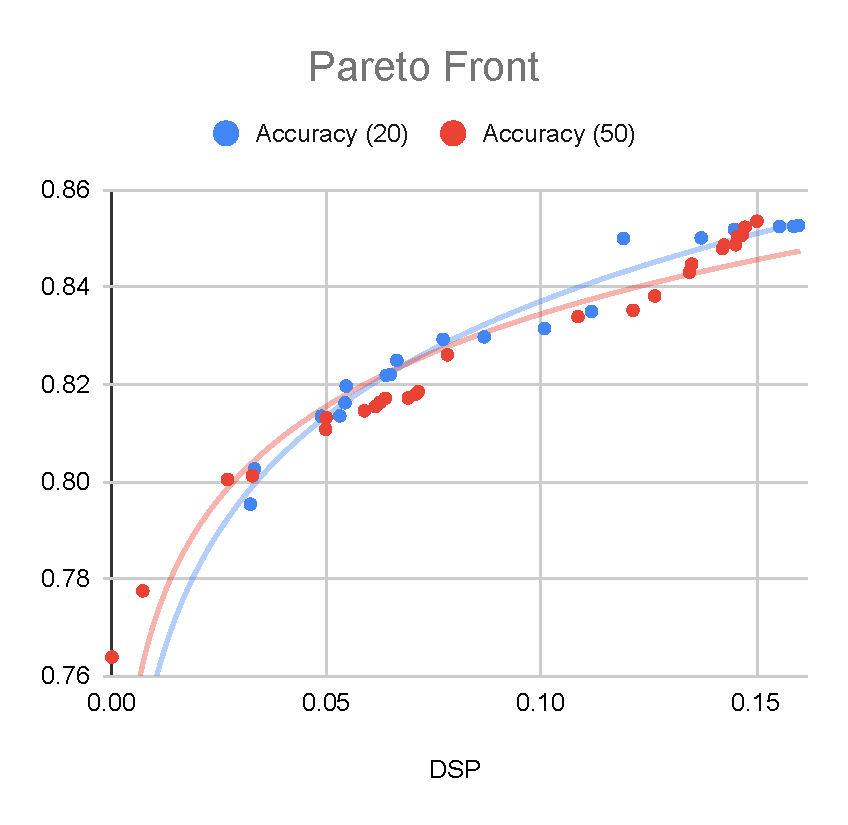
\includegraphics[width=0.65\textwidth]{Graphics/pareto-front.pdf}
    \end{center}
    \caption{Aproximación del \emph{Frente Pareto} encontrada por el sistema.}
    \label{fig:pareto-dsp-vs-acc}
\end{figure}


\todo[inline]{Falta poner un párrafo aqui (justo como hiciste en el anologo de la primera etapa) que dice que a continuacion en la seccion de discusión se dan insights al respecto. O lo pones así, o como una oración al final del unico párrafo de esta seccion}


\subsection{Discusión}\label{section:discussion-second-phase}

Los resultados observados en la tabla~\ref{table:second-phase-vs-all} muestran que nuestro sistema es sumamente competitivo y en la mayoría de los casos superior que el resto de los métodos de mitigación de sesgos con los cuales es comparado.
El enfoque propuesto obtiene mejores resultados que todos los métodos agnósticos al modelo con los que fue comparado, estos son, \emph{FERM Preprocesamiento}, \emph{SMOTE} y \emph{FairBO}.
Comparado con métodos que modifican directamente el proceso de optimización de los modelos para ajustarlos a los objetivos de equidad, nuestro sistema también muestra resultados satisfactorios, siendo solamente superado por \emph{FERM}, y aun en este caso se mantiene muy competitivo.
Esto ratifica el potencial de nuestro enfoque multiobjetivo para encontrar modelos que sean efectivos a la vez que son justos de acuerdo a la métrica de equidad seleccionada.
Particularmente interesante es el hecho de que se obtienen resultados competitivos, incluso superiores a las estrategias que son \emph{ad-hoc} y directamente modifican el método de optimización del modelo en cuestión.
Solo el caso de \emph{FERM} obtiene resultados mejores a los nuestros como se esperaba inicialmente dado que las restricciones de equidad son mantenidas durante el proceso de optimización.
Sin embargo la diferencia es modesta y nuestro sistema logra ser muy competitivo mientras que es mucho más versátil al mantenerse agnóstico al modelo y método de entrenamiento.
Adicionalmente es importante destacar que \emph{Adversarial debiasing} (tercera fila) utiliza métodos de aprendizaje profundo, dígase \emph{Redes Neuronales Adversariales}, mientras que nuestro sistema no incluye este tipo de modelos que sabemos son mas poderosos en muchos escenarios.

La tabla~\ref{table:secod-phase-vs-fbo} compara nuestra propuesta con \emph{Fair Bayesian Optimization}.
\emph{FBO} consiste en un proceso de ajuste de hiperparámetros mediante optimización bayesiana para lograr los resultados de equidad requeridos.
La flexibilidad de este método le permite hacer cumplir restricciones sobre diferentes métricas de equidad simultáneamente, por lo que nuestro sistema es comparado en este escenario con dicha propuesta.
Como se puede observar nuestro sistema obtiene mejores resultados que la alternativa en la mayoría de los casos.
Incluso para configuraciones de \emph{FBO} basadas en redes neuronales, nuestro sistema fue capaz, una vez más de obtener significativamente mejores resultados aun cuando nuestras configuraciones no utilizan algoritmos de aprendizaje profundo.
Debido a la forma en que \emph{FBO} funciona, requiere un umbral para cada métrica y la única garantía que provee es que dichas métricas de equidad se mantendrán dentro de esta región factible luego de ajustar los hiperparámetros.
En cambio nuestro enfoque no necesita que el usuario indique el umbral admisible para las métricas de equidad y es capaz de explorar los diferentes balances entre las diferentes métricas (tanto de equidad como de precisión) y permitir al usuario seleccionar el que considere conveniente.
Adicionalmente puede observarse como a pesar de que nuestro sistema obtiene resultados muy cercanos al umbral para \emph{statistical parity}, este a la vez obtiene considerablemente mejores resultados en el resto de las métricas de equidad.
Esto quiere decir que nuestro sistema es capaz de mostrar resultados sumamente satisfactorios utilizando no solo una, pero varias métricas de equidad simultáneamente.
Una vez más, la configuración que obtiene mejores resultados que los nuestros no supera nuestro modelo significativamente, además, se conoce que el algoritmo utilizado por este modelo (\emph{XGBoost}) no forma parte del conjunto de algoritmos disponibles a AutoGOAL en nuestra configuración, lo que sugiere que la comparativa podría haber sido similar al resto de los casos de haber tenido acceso al mismo.

La tabla~\ref{table:second-phase-vs-mobo} muestra una comparación con otros métodos de optimización multiobjetivo que han sido aplicados en la literatura al problema de mitigación de sesgos.
Una vez mas nuestro sistema muestra ser competitivo en este ámbito, encontrando diferentes balances entre precisión y equidad.
En todos los casos nuestro sistema supera los sistemas alternativos.
Además se puede observar como nuestro sistema es capaz de encontrar soluciones que a pesar de que ceden de forma mínima sus valores de equidad son capaces de lograr significativamente mejores valores de precisión.
Esto habla entre otras cosas de la habilidad de nuestro enfoque para cubrir diferentes regiones del \emph{Frente Pareto}.

De forma general, como se ha podido observar, el sistema muestra un elevada capacidad para encontrar balances satisfactorios entre las métricas de equidad deseadas y la pérdida de los modelos.
Todo esto mientras se mantiene extremadamente versátil, siendo agnóstico al modelo que se utilice, a las métricas que se desean optimizar, incluso a la naturaleza del problema que se desea resolver.
